% Options for packages loaded elsewhere
%\PassOptionsToPackage{unicode}{hyperref}
\PassOptionsToPackage{hyphens}{url}
%
\documentclass[11pt]{article}
\usepackage{lmodern}
\usepackage{amssymb,amsmath}
\usepackage{ifxetex,ifluatex}
\ifnum 0\ifxetex 1\fi\ifluatex 1\fi=0 % if pdftex
  \usepackage[T1]{fontenc}
  \usepackage[utf8]{inputenc}
  \usepackage{textcomp} % provide euro and other symbols
\else % if luatex or xetex
  \usepackage{unicode-math}
  \defaultfontfeatures{Scale=MatchLowercase}
  \defaultfontfeatures[\rmfamily]{Ligatures=TeX,Scale=1}
\fi
% Use upquote if available, for straight quotes in verbatim environments %
\IfFileExists{upquote.sty}{\usepackage{upquote}}{}
\IfFileExists{microtype.sty}{% use microtype if available
  \usepackage[]{microtype}
  \UseMicrotypeSet[protrusion]{basicmath} % disable protrusion for tt fonts
}{}
\makeatletter
\@ifundefined{KOMAClassName}{% if non-KOMA class
  \IfFileExists{parskip.sty}{%
    \usepackage{parskip}
  }{% else
    \setlength{\parindent}{0pt}
    \setlength{\parskip}{6pt plus 2pt minus 1pt}}
}{% if KOMA class
  \KOMAoptions{parskip=half}}
\makeatother
\usepackage{xcolor}
\IfFileExists{xurl.sty}{\usepackage{xurl}}{} % add URL line breaks if available
%\IfFileExists{bookmark.sty}{\usepackage{bookmark}}{\usepackage{hyperref}}
\urlstyle{same} % disable monospaced font for URLs
\usepackage[margin=1in]{geometry}
\usepackage{color}
\usepackage{fancyvrb}
\newcommand{\VerbBar}{|}
\newcommand{\VERB}{\Verb[commandchars=\\\{\}]}
\DefineVerbatimEnvironment{Highlighting}{Verbatim}{commandchars=\\\{\}}
% Add ',fontsize=\small' for more characters per line
\usepackage{framed}
\usepackage{changepage}
\usepackage{graphicx,grffile}
\makeatletter
\def\maxwidth{\ifdim\Gin@nat@width>\linewidth\linewidth\else\Gin@nat@width\fi}
\def\maxheight{\ifdim\Gin@nat@height>\textheight\textheight\else\Gin@nat@height\fi}
\makeatother
% Scale images if necessary, so that they will not overflow the page
% margins by default, and it is still possible to overwrite the defaults
% using explicit options in \includegraphics[width, height, ...]{}
\setkeys{Gin}{width=\maxwidth,height=\maxheight,keepaspectratio}
% Set default figure placement to htbp
\makeatletter
\def\fps@figure{htbp}
\makeatother
\setlength{\emergencystretch}{3em} % prevent overfull lines
\providecommand{\tightlist}{%
  \setlength{\itemsep}{0pt}\setlength{\parskip}{0pt}}
%\setcounter{secnumdepth}{-\maxdimen} % remove section numbering
%C'est fini pour les packages pour le code R 
\usepackage[francais]{babel} 
\usepackage[T1]{fontenc}
\usepackage{a4wide}

\pagestyle{myheadings}
\usepackage{fancyhdr}
\usepackage{amsmath,amsfonts,amssymb}
\pagestyle{plain}
\usepackage{subcaption}
\usepackage{xcolor} 
\usepackage{mdframed}
\usepackage{color,soul}
\sethlcolor{yellow}
\pagestyle{fancy}
%\fancyhead[C]{\thechapter}
%\fancyhead[CE]{contenu}
%\fancyfoot[c]{\thepage}
\renewcommand{\headrulewidth}{1pt}
%\fancyhead[C]{ } 
\fancyhead[L]{Classification supervisée de personnages}
\renewcommand{\footrulewidth}{1pt}
\fancyfoot[C]{\textbf{\thepage}} 
\fancyfoot[L]{ Master 1 -- MIND}
\fancyfoot[R]{ 2020/2021}

%\usepackage{float} 
\usepackage{mathtools}
%\usepackage{algorithm}
\usepackage[]{algorithmic}
\usepackage{algorithm2e}
%--
%setcounter{secnumdepth}{4}
%\newcommand{\myparagraph}[1]{\paragraph{#1}\mbox{}\\}
%\documentclass[12pt]{book}
\usepackage[utf8]{inputenc}
%\usepackage[frenchb]{babel}
%\usepackage{lipsum}
\usepackage{graphics}
\usepackage{graphicx}
\usepackage{xcolor, soul}
\sethlcolor{yellow}
\usepackage[french]{minitoc}
\usepackage[colorlinks = true,
            linkcolor = blue,
            urlcolor  = black,
            citecolor = black]{hyperref}
%\usepackage{minitoc}

\usepackage{float}
\usepackage[textwidth=1.5cm, textsize=scriptsize]{todonotes}
\newcommand{\tif}[1]{\todo[color=blue!20]{\textbf{ Tif:} #1}}

\begin{document}
\thispagestyle{empty}
\begin{titlepage}
  \begin{sffamily}
  \begin{center}

    % Upper part of the page. The '~' is needed because \\
    % only works if a paragraph has started.
    

   

    
    % Title
    
    
\includegraphics[width= 10 cm]{./figures/untitled.png}
    \\[3cm]
    \textsc{Master 1 MIND }\\
    \vspace{0.4cm}
    \textsc{Rapport de projet }\\
    \vspace{1cm}
    
    \hrule
    \vspace{0.4cm}
    { \huge \scshape \textbf{Classification supervisée de personnages sur la saga Harry Potter}}
    \vspace{0.4cm}
    \hrule
    \vspace{4 cm}
    
    

    % Author and supervisor
    \begin{minipage}{0.5\textwidth}
      \begin{flushleft} \Large
        \emph{Auteurs : }\\
        \textsc{Bouthayna HAYOU}\\
        \textsc{Jihène BELGAIED }\\
        \textsc{Jalal SAKHER}\\
    
      \end{flushleft}
    \end{minipage}
    \begin{minipage}{0.43\textwidth}
      \begin{flushright} \Large
        \emph{Encadrants : }\\
    \textsc{Florent BASCOU}\\
    \textsc{Tiffany CHERCHI}
      \end{flushright}
    \end{minipage}

    \vfill

  \end{center}
  \end{sffamily}
\end{titlepage}

\newpage


\thispagestyle{plain} % empty
\mbox{}

\renewcommand{\contentsname}{Sommaire}
\tableofcontents
\newpage

\section{Introduction}

Nous exploitons dans ce projet des données issues des 3 premières films de la saga Harry Potter à savoir « Harry Potter à l'école des sorciers », « Harry Potter et la Chambre des Secrets », « Harry Potter et le prisonnier d’Azkaban » ainsi qu'un dataframe donnant différentes caractéristiques des personnages; caractérisitques que nous décriveront par la suite.\\
Ajouter 
L’objectif est de répondre à la question suivante : est-il possible de prédire l’appartenance d’un nouveau personnage à l’une des 4 maisons Poudlard ?

% Quelle contexte, quelle problématique (cf commentaire), quelles pre-traitement des données, quelles méthodes statistiques, quelles difficultés statistiques.
% {Penser à faire une introduction globale. Vous pouvez déjà répondre au premier point.}
% Rajouter dans intro : les script des trois films seront préparés de la même façon. Par contre pour la suite, nous utiliseront les script des 2 premiers pour entraîner notre modèle pour ensuite le tester sur le troisième. 

\newpage

%------------------------------------------------------%
%------------------------------------------------------%
\section{Présentation des données}
%------------------------------------------------------%
%------------------------------------------------------%


Nous manipulons dans notre étude des jeux de données qui présentent différentes variables.\\

Dans le but de cerner le contexte de cette dernière liée au monde de la magie d'Harry Potter, nous allons dans un premier temps les présenter et les décrire. Nous pourrons de cette façon comprendre les rôles de ces varaibles dans l'analyse que nous allons menner. \\
Nos données brutes de départ sont composées de 4 dataframes.


%------------------------------------------------------%
\subsection{Les scripts}
%------------------------------------------------------%

Les 3 dataframes contiennent les scripts des 3 premiers films d'Harry Potter. Les variables sont donc logiquement :

\begin{itemize}
	\item Character : Nom des personnages
	\item Sentence : Paroles prononcés lors du film. 
\end{itemize}


%------------------------------------------------------%
\subsection{Caractéristiques des personnages}
%------------------------------------------------------%

Les données "Characters.csv" contiennent différentes caractérisitques spécifiques à chaucun des personnages :

\tif{pour avoir une liste non numérotée, vous pouvez utiliser l'environnement 'itemize' qui revient automatiquement à la ligne avec des tirets. Je vous laisse changer les autres.}
\begin{itemize}
	\item Name : Nom des personnages
	\item Gender : Genre du personnage
	\item House : Appartenance à l'une des 4 maisons Poudlard
	\item Blood Status : Statuts de sang (au nombre de 5)
	\item Loyalty : Loyauté pour une entité
	\item Skills : Qualités reconnues des personnages
\end{itemize}


%------------------------------------------------------%
%------------------------------------------------------%
\section{Préparation de données}
%------------------------------------------------------%
%------------------------------------------------------%


Dans cette partie, nous commençons par la préparation de données. Elle désigne les opérations de nettoyage et transformation qui doivent être appliqués aux données brutes avant leur traitement et analyse. Cette opération représente une étape importante avant le traitement proprement dit, qui implique souvent de reformater et corriger les données et de combiner des datasets pour enrichir certaines données.

%------------------------------------------------------%
\subsection{Nettoyage de données}
%------------------------------------------------------%

Pendant cette première phase, nous vérifions les données brutes avec soin afin de déceler d’éventuelles erreurs. L’objectif est d’éliminer les données de mauvaise qualité (redondantes, incomplètes ou incorrectes) (Jalal needs to describe what he did)


%------------------------------------------------------%
\subsection{Manipulation de texte}
%------------------------------------------------------%

L'analyse naturelle du langage (NLP: Natural Language Processing) nécessite un prétraitement du texte en le transférant du langage humain vers un format lisible par machine pour un traitement ultérieur.\\

Dans cette deuxième phase, nous nettoyons donc les discours de chaque personnage dans les 3 films. Cette opération est faite, à l'aide du package python NLTK (Natural Language Toolkit), en trois étapes :\\


\subsubsection{Tokenization}

La tokenisation consiste à découper un texte en morceaux. Ces morceaux pourraient être des phrases, des symboles ou des mots. C’est cette dernière option que l’on va choisir, plus simple pour retirer les stop words mais surtout pour mener à bien notre analyse statistique en seconde partie. \\


\subsubsection{Stemming}

Pour réduire la complexité d’un texte, on peut tirer parti de « classes d’équivalence » : on peut considérer que différentes formes d’un même mot (pluriel, singulier, conjugaison) sont équivalentes et les remplacer par une même forme dite canonique. Il existe deux approches dans le domaine, la racinisation et la lemmatisation :

\tif{pour avoir une listenumérotée, vous pouvez utiliser l'environnement 'enumerate'. Je vous laisse changer les autres.}
\begin{enumerate}
	\item La racinisation est simple à mettre en œuvre car elle peut s’appuyer sur des règles simples pour extraire la racine d’un mot, c’est-à-dire, le tronquer de toute déclinaison, accords et dérivations. Mais cette approche a ses défauts puisqu’elle peut changer les noms des personnages (Harry/Harri).
	\item La lemmatisation requiert la connaissance des statuts grammaticaux (exemple : chevaux devient cheval).
\end{enumerate}
    
    On fait donc le choix de la lemmatization dans notre méthodologie, qui consiste à ramener un terme, quelque soit ses accords et déclinaisons à sa forme la plus simple.Cette méthode nous permmettra d'avoir moins d'erreurs d'interprétation par la suite.\\ 

\subsubsection{stop-words removal}

Cette étape consiste à enlever les mots communs comme les pronoms, prepositions, conjonctions...


%------------------------------------------------------%
\subsection{Visualisation et analyse de données}
%------------------------------------------------------%

Dans cette partie, nous exploitons les résultats obtenus de la partie prétraitement afin d'étudier et d'extraire les variables explicatives qui influence principalement sur notre variable cible, dans ce cas l’appartenance à une maison Poudlard.\\

\tif{Utilisez l'environnement 'figure'. Le titre se met grâce à 'caption' et pour y faire référence on utilise 'label'. Je vous laisse changer les autres.}

\begin{figure}[H]
\centering
    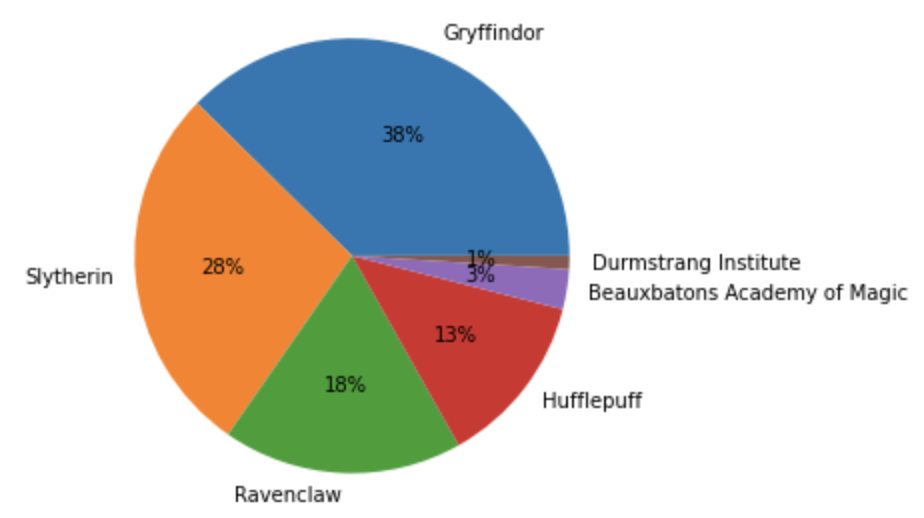
\includegraphics[width=11 cm]{./figures/rep.png}
    \caption{Répartition des personnages par maison}
    \label{Répartition}
    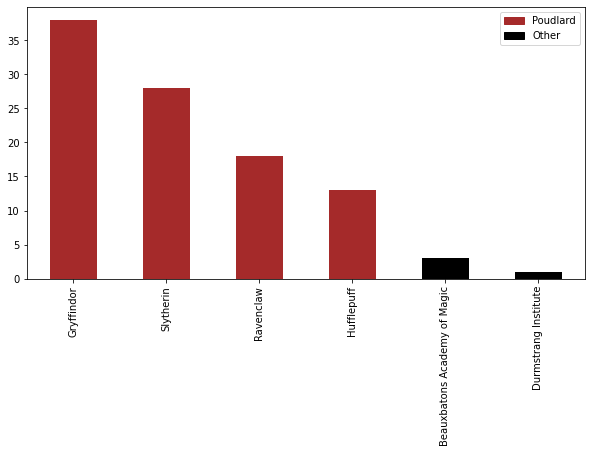
\includegraphics[width=11 cm]{./figures/houses.png}
    \caption{Regroupement des maisons}
    \label{Regroupement}
\end{figure}

\tif{Vous pouvez  aligner plusieurs images, si c'est votre intention}

\begin{figure}[H]
    \centering
    \begin{subfigure}[b]{0.6\textwidth}
        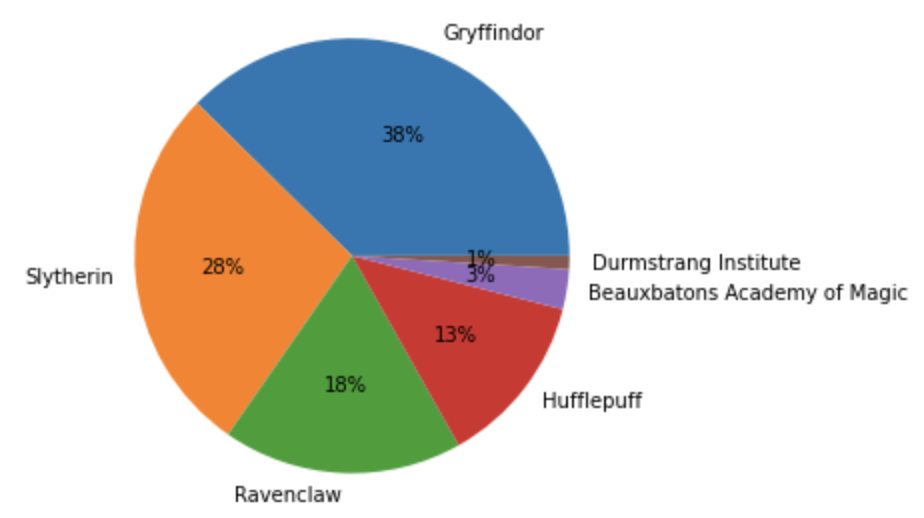
\includegraphics[width=5cm]{./figures/rep.png}
    \end{subfigure}
    \begin{subfigure}[b]{0.3\textwidth}
        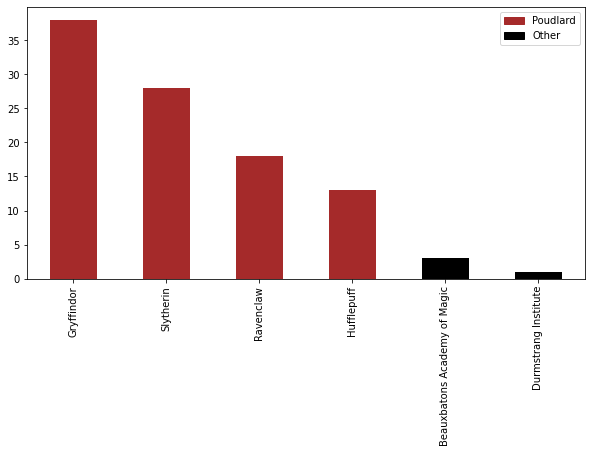
\includegraphics[width=5cm]{./figures/houses.png}
    \end{subfigure}
    \caption{2 images side by side, OMG}
\end{figure}

La \autoref{Répartition} représente la répartition des personnage selon les maisons. Nous remarquons que 66\% des personnages appartiennent aux maisons Gryffindor et Slytherin. En outre, nous constatons que le pourcentage des personnages des maisons "Beaubatons" et "Drumstrang" ne dépassent pas 4\%. Selon la Figure 3, ces dernières appartiennent à des écoles différentes des autres maisons qui font partie de l'école Poudlard.\\ 

Nous étudions dans la suite le lien entre les caractéristiques des personnages; principalement le sexe et le statut sanguin, et l'appartenance à une maison.

\begin{figure}
\centering
    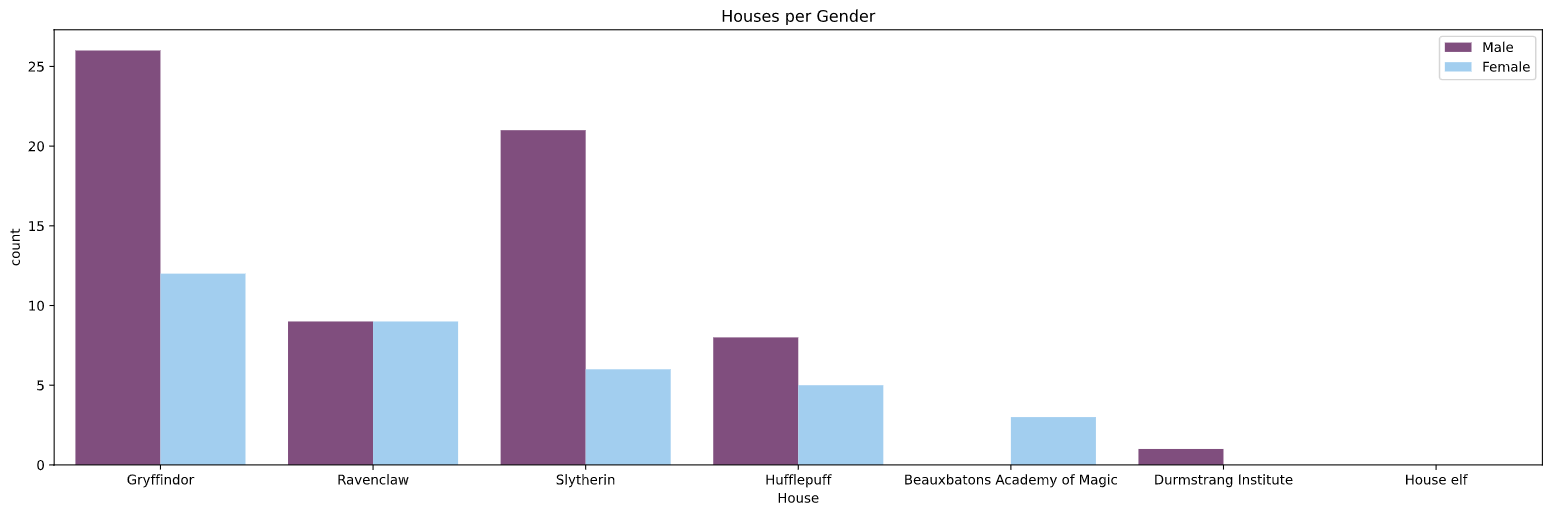
\includegraphics[width= 15 cm]{./figures/Houses per gender 1.png}
     \caption{Répartition des genres par maison}
\end{figure}

La Figure 4 représente la répartition des personnages par sexe dans chaque maison. Nous remarquons que les maisons Poudlard contiennent des garçons et des filles, alors que les autres écoles sélectionnent selon le sexe.\\

La Figure 5 décrit les différents statuts sanguins présents dans chaque maison. 

\begin{center}
    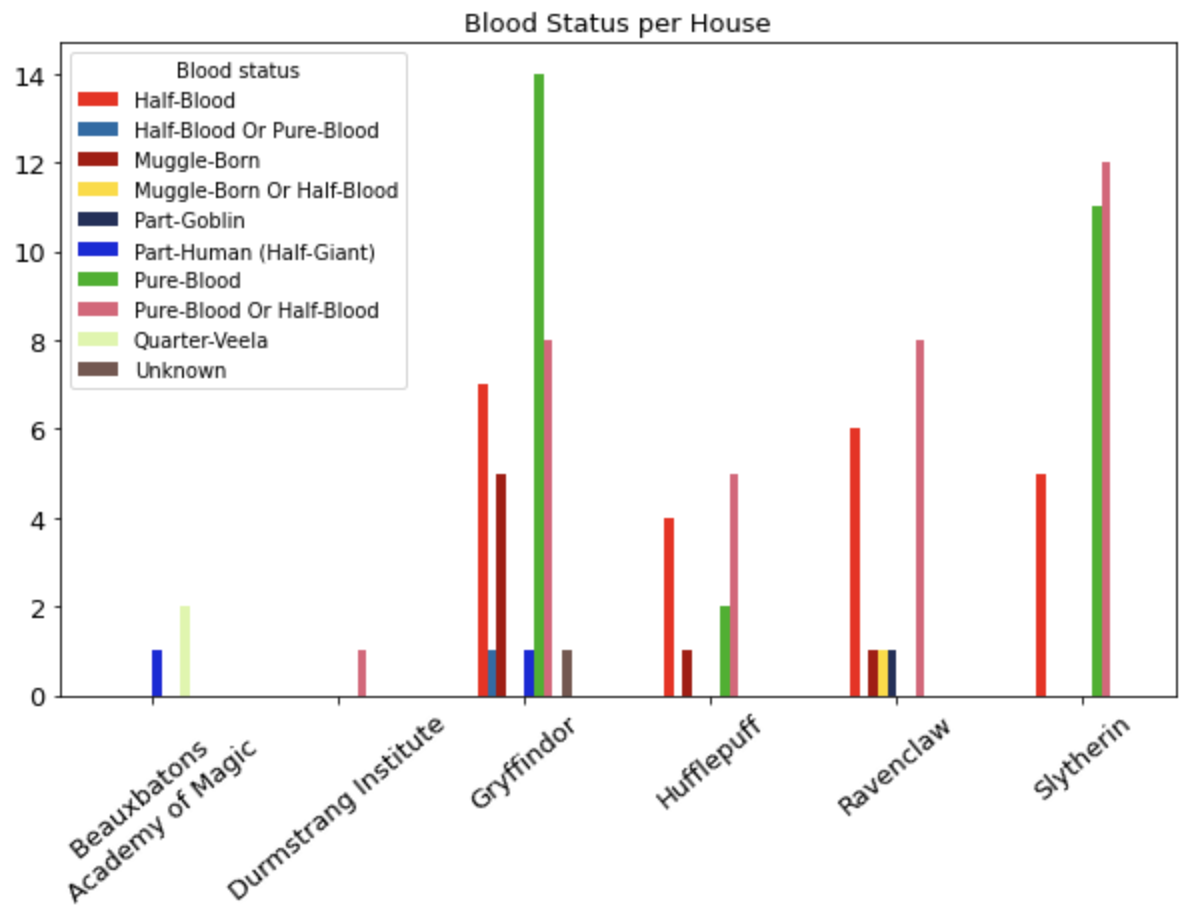
\includegraphics[width= 15 cm]{./figures/blood_status.png}
     \text{Figure 5 - Repartition du statut de sang par maison}
\end{center}

Nous remarquons que le sang de type "Pure-Blood" et "Half-Blood" dominent toutes les maisons de l'école Poudlard. De plus, dans cette école, le type "Part-Human" caractérise une partie de personnages appartenant à la maison Gryffindor. La figure montre aussi que le type "Quarter-Veela" est absent de toutes les maisons sauf "Beauxbatons". Nous pouvons prévoir que le statut sanguin est une variable significative dans la classification des personnages.\\

L'analyse émotionnelle représente une des applications les plus utilisées dans le NLP. Dans cette optique, nous exploitons le traitement de texte effectué précédemment pour étudier le degré d'affect émotionnel dans le discours des personnages.\\

NRCLeX est une bibliothèque python qui contient un dictionnaire des affects avec environ 27 000 mots et qui se base sur le lexique des affects du Conseil National de Recherches du Canada (CNRC) et sur les ensembles des synonymes Wordnet de la bibliothèque NLTK. Dans le cadre de ce projet, nous utilisons cette bibliothèque pour générer les émotions à partir d'un corps de texte vu la difficulté de construire un modèle dédié à cette analyse. Les affects émotionnels mesurés par NRCLeX sont : la peur, la colère, l'anticipation, la confiance, la surprise, la positivité, la négativité, la tristesse, le dégoût et la joie.\\

La Figure 6 représente les différentes émotions pour chaque maison mesurées à partir des personnages qui y appartiennent. 

\begin{center}
    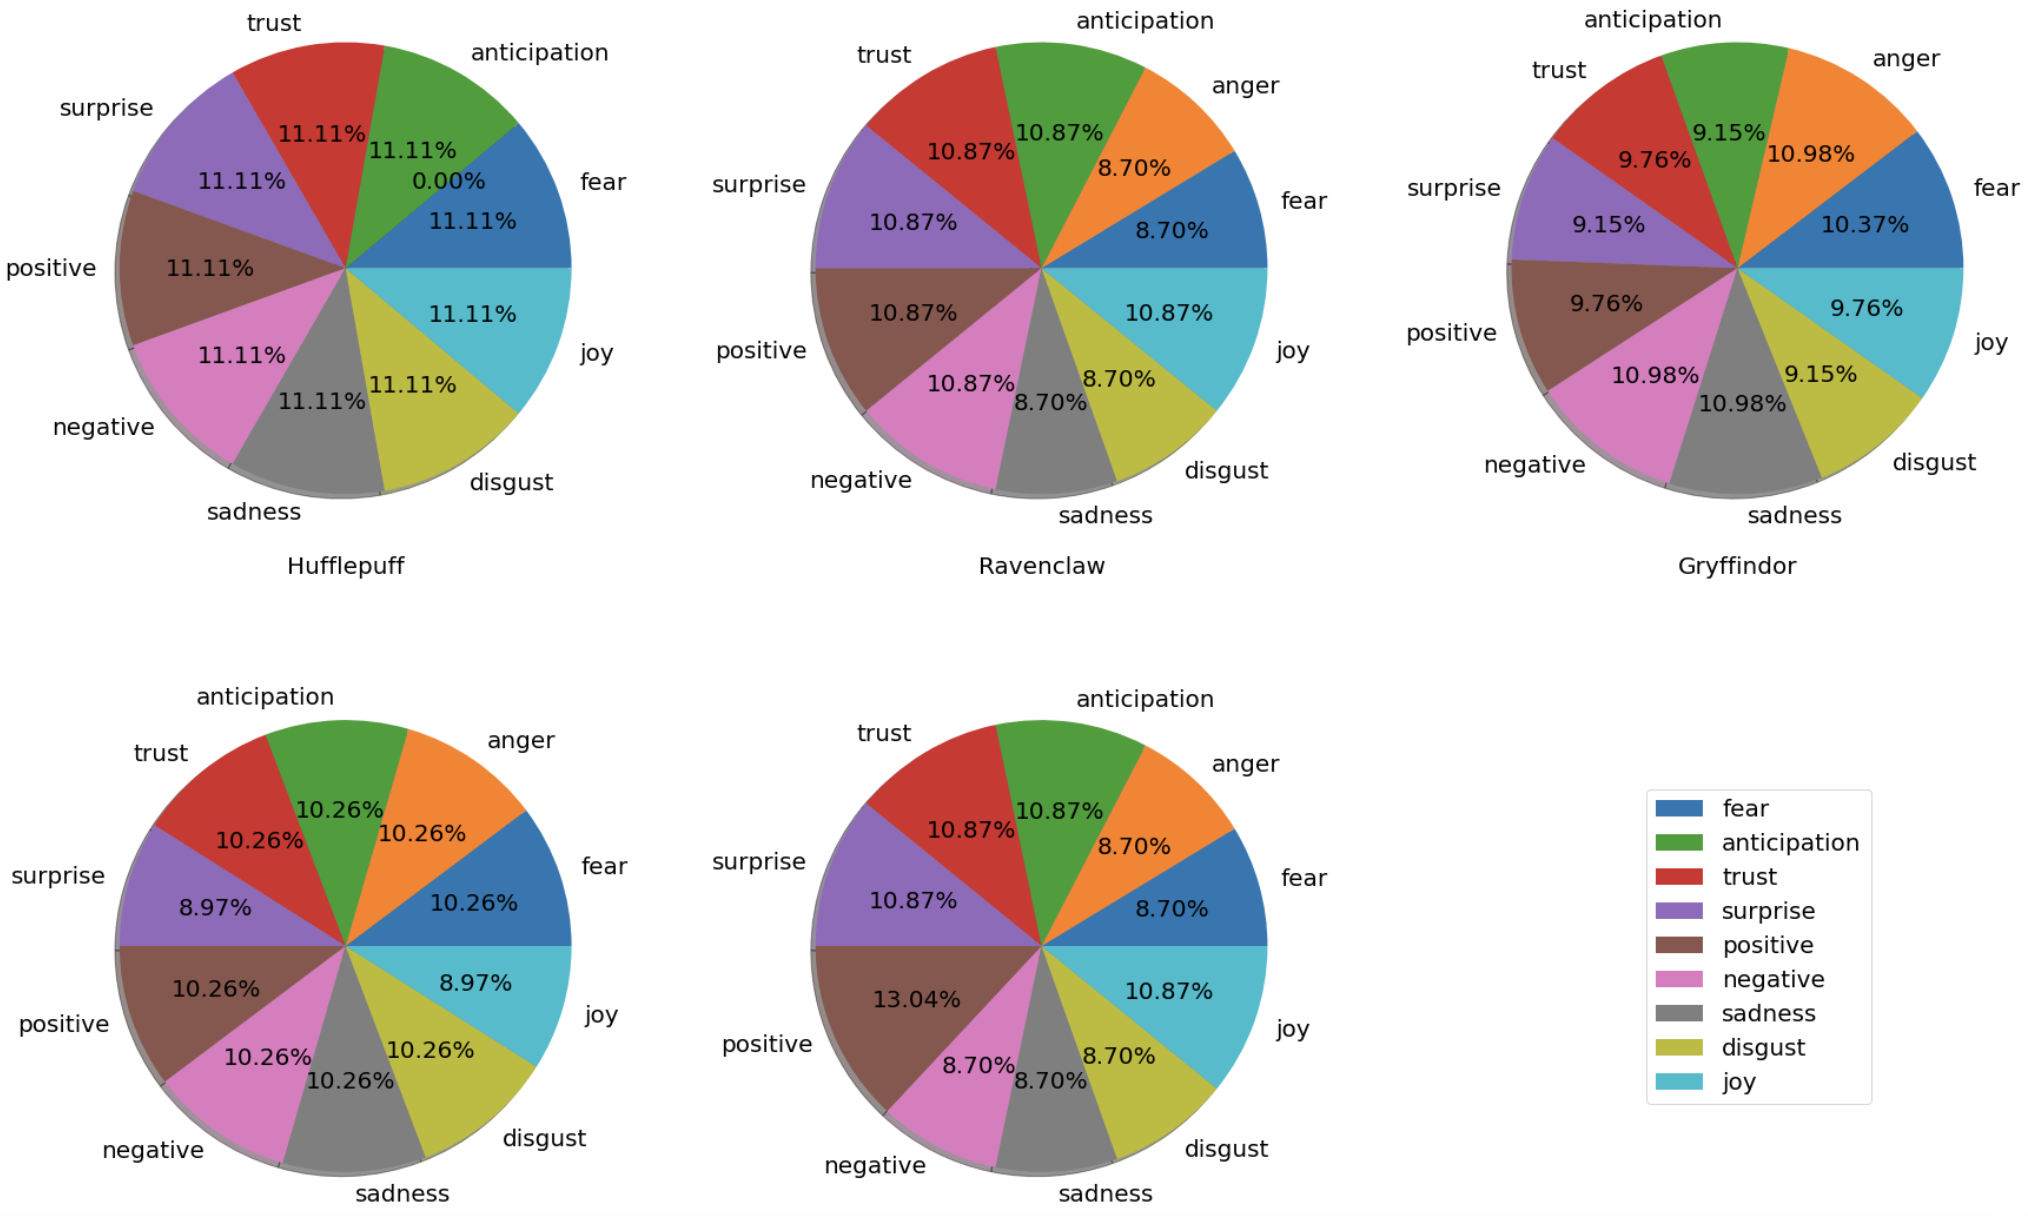
\includegraphics[width= 17 cm]{./figures/emotions_houses.png}
    \text{Figure 6 - Analyse des émotions par maison}
\end{center}

Nous remarquons que la colère est une émotion non-exprimée par les personnages de la maison "Hufflepuff". De plus, le comportement émotionnel général de la maison "Slytherin" s'oppose à celui de "Gryffindor"; principalement au niveau des émotions "positive", "négative", "sadness" et "anger".D'autre part, ce comportement est quasiment similaire à celui de la maison "Ravenclaw" sauf au niveau de la positivité et la négativité.\\

\textbf{\textit{Remarque :}} Nous utilisons les émotions exprimées par personnage comme variables explicatives dans la matrice de design.

%------------------------------------------------------%
\subsection{Matrice de design}
%------------------------------------------------------%

- Ces informations, ainsi collectées nous servrons à former une matrice.


%------------------------------------------------------%
%------------------------------------------------------%
\section{Analyse statistique}
%------------------------------------------------------%
%------------------------------------------------------%


Dans cette séction nous examinons plusieurs stratégies pour construire (ou assembler) des classifieurs performants à partir de classifieurs de base plus modestes. On parle de « méthodes d’agrégation ». 
Nous allons commencer par une discussion des avantages et des défauts des arbres de décision, surtout le problème des estimateurs de variance élevée. Ensuite nous présenterons les deux approches classiques conçues pour répondre à ce problème : le « Bagging » et les « Forêts aléatoires » et nous finirons par expliquer le Boosting, qui permet de combiner la sortie de plusieurs classifieurs simples pour en obtenir un meilleur résultat.


%------------------------------------------------------%
\subsection{Titre ?}
%------------------------------------------------------%

\subsubsection{Estimateurs de variance élevée}

$\bullet$ Avantages et inconvénients : 

Comparativement à d'autres méthodes d’apprentissage statistique, les arbres de décision présentent plusieurs avantages :\\
•	La simplicité de compréhension et d'interprétation. 
C'est un modèle boîte blanche : si l'on observe une certaine situation sur un modèle, celle-ci peut-être facilement expliquée à l'aide de la logique booléenne, au contraire de modèles boîte noire comme les réseaux neuronaux, dont l'explication des résultats est difficile à comprendre.\\
•	Peu de préparation des données (pas de normalisation, de valeurs vides à supprimer, ou de variable muette).\\
•	Il est possible de valider un modèle à l'aide de tests statistiques, et ainsi de rendre compte de la fiabilité du modèle.\\
•	Performant sur de grands jeux de données: la méthode est relativement économique en termes de ressources de calcul.\\
•	Ils sont capables de gérer des problèmes multi-classes.\\

> Inconvénients : 

•	Il est possible que les arbres générés ne soient pas équilibrés (le temps de parcours n’est donc plus logarithmique). Il est donc recommandé d’équilibrer la base de données avant la construction, pour éviter qu’une classe domine (en termes de nombre d’exemples d’apprentissage).\\
•	Sur-apprentissage : Il est possible que possible les arbres générés sont trop complexes et généralisent mal (solution : élagage, le contrôle de la profondeur de l’arbre et de la taille des feuilles).\\
•	Il est aussi possible que les arbres soent instables : des changements légers dans les données produisent des arbres très différents. Les changements des nœuds proches de la racine affectent beaucoup l’arbre résultant. On dit que les arbres produisent des estimateurs de variance élevée.\\

Le besoin de répondre à ce troisième problème, qui n’admet pas de solution par optimisation algorithmique, a conduit aux approches de type Bagging et « Forêts aléatoires ».\\

L’idée derrière et celle de la Réduction de variance : on utilise pour cela la moyenne de plusieurs estimateurs, calculés sur des données légèrement différentes, en somme utiliser le hasard pour améliorer les performances des algorithmes de base (qui sont les arbres de décision CART).\\

Définissons désormais le Bagging : 

\subsubsection{Bagging} 

Le Bagging est née du Bootstrap Agregating.

Nottons quelques nottations avant de définir son algorithme :

- $(x_{i},y_{i}),x_{i} \in \mathbb{R}^p, y_{i} \in \mathbb{R}^p, i=1,..,N$ : données d'apprentissage \\
- $A_{1},...,A_{p}$ sont les attributs de nos données\\
- $y_{i}$ : étiquettes des classes : peuvent être des valeurs continues ou discrètes.\\
- $x_{i}=(a_{1},..,a_{p}$\\
- $G(x)$ un modèle de prédiction appris sur un échantillon de données $z ={(x_{i},y_{i})_{i=1}}$ (revoir nottation)\\


$\bullet$ Algorithme bagging : \\

1. On tire au hasard dans la base d’apprentissage B échantillons avec remise $z_{i},i=1,…,B$ (chaque échantillon ayant n points)  appelés échantillons bootstrap ;\\

2. Pour chaque échantillon i on calcule le modèle $G_{i}(x)$ ;\\

3. Classement : agrégation par vote : 
$$G(x)=Votemajoritaire(G_{1}(x),…,G_{B}(x))$$

N.B : L'erreur OOB (Out Of Bag) est un critère de performance pour le calcul de B. Cette erreur correspond à la moyenne des erreurs des classifieurs $G_{i}$ tel que $x_{i} \notin	z_{i}$. ($x_{i}$ ne fait pas partie de l'échantillon bootstrap de $G_{i}$). Lorsque l'erreur se stabilise et ne descend plus on choisit B.\\

$\bullet$ Défauts du bagging : \\

Les estimateurs $G_{i}$ sont calculés sur des échantillons qui se recouvrent fortement (tirage avec remise) et donc ils sont corrélés.Ils ne sont donc pas indépendants mais plutôt corrélés.\\

(inclure formule corrélation, variance + explication)

Les forêts aléatoires améliorent ce modèle en baissant la corrélation entre les $G_{i}$ et ce par la randomisation.

Nous allons définir les "forêts aléatoires"

\subsubsection{ "Forêts Aléatoires" (Random Forest)}

Random Forest est un algorithme qui se base sur l’assemblage d’arbres de décision. Il a été proposé par par Leo Breiman en 2001.\\


$\bullet$ Principe de fonctionnement : \\
Un random forest est constitué d'un ensemble d'arbres de décision indépendants.Chaque arbre dispose d'une vision parcellaire du problème du fait d'un double tirage aléatoire :

- Le tree bagging : un tirage aléatoire avec remplacement sur les observations (les lignes de notre matrice). 

- Le feature sampling: un tirage aléatoire sur les variables (les colonnes de notre matrice).\\

A la fin, tous ces arbres de décisions indépendants sont assemblés. La prédiction faite par le random forest pour des données inconnues est alors la moyenne (dans notre cas le vote car nous traitons un problème de classification) de tous les arbres.

L'idée de base de cet algorithme est assez intuitive. A titre d’exemple, si vous voulez connaître les performances d’un produit et que vous hésitez à l’acheter vous irez lire plusieurs avis afin de prendre une décision. Effectivement, un seul avis ne suffit pas en général pour prendre la meilleure décision.

Le random forest fonctionne sur ce même principe : plutôt que d'avoir un estimateur complexe capable de tout faire, le random forest utilise plusieurs estimateurs simples (de moins bonne qualité individuelle, nous verrons la raison plus tard). 

Chaque estimateur a une vision parcellaire du problème. Ensuite, l'ensemble de ces estimateurs est réuni pour obtenir la vision globale du problème. C'est l'assemblage de tous ces estimateurs qui implique une meilleure performance de la prédiction.


De plus comme nous l'avons dit plus tôt cette méthode permet de réduire la corrélation entre les arbres $G_{i}$ car :\\

- Ils sont construits sur des échantillons différents
- Ils sont appris sur un ensemble différent d’attributs


Pour mieux comprendre la préocédure reprennant son algorithme : 


$\bullet$ Algorithme "forêts aléatoires" :

1.  On tire au hasard dans la base d’apprentissage B échantillons avec remise $z_{i},i=1,…,B$ (chaque échantillon ayant n points). Jusque là, on opère comme le bagging.

2. La différence arrive ici : pour chaque échantillon i on construit un arbre CART $Gi(x)$ selon un algorithme légèrement modifié : a chaque fois qu’un nœud doit être coupé (étape “split”) on tire au hasard une partie des attributs (q parmi les p attributs) et on choisit le meilleur découpage dans ce sous-ensemble.

3. On finit comme pour le bagging par une aggrégation par vote :
$$G(x)=Votemajoritaire(G_{1}(x),…,G_{B}(x)).$$

N.B : 
- On se limite à un petit nombre d'arbres, ce qui n'est pas le cas du bagging qui demande des arbres profonds afin de réduire leurs corrélation (risque du overfitting)

- Chaque arbre est petit donc moins performant mais l'aggréation des petits arbres (les attributs sont contenus dans plusieurs arbres) implique une bonne performance du modèle.


%------------------------------------------------------%
\subsection{Choix de la méthode pour notre étude : }
%------------------------------------------------------%

Le premier critère que nous avons opté dans le choix des méthodes statistiques est le compromis entre l'interprétabilité et l'efficacité de la méthode.

\begin{center}
       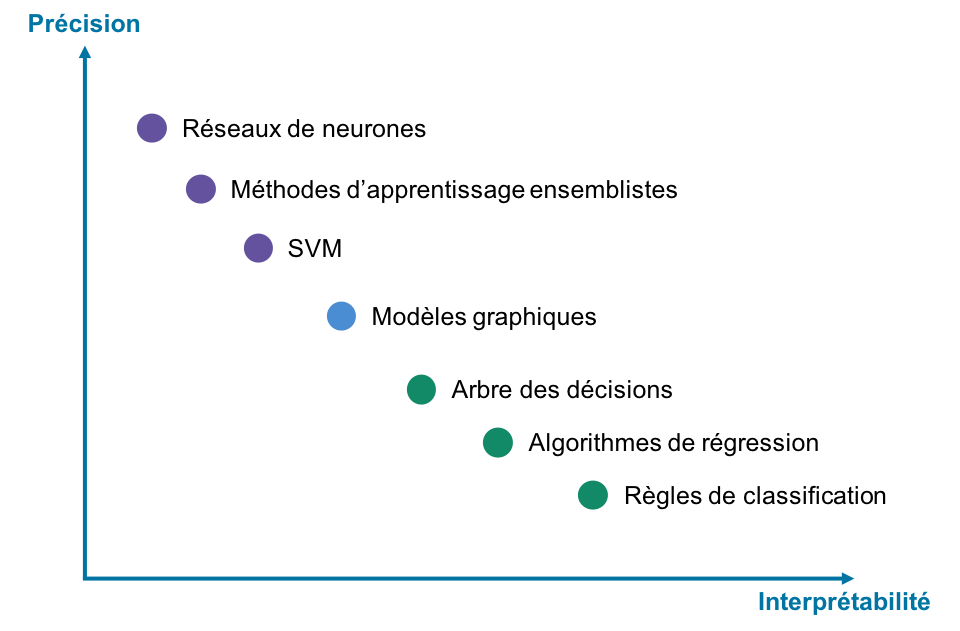
\includegraphics[width=13cm]{./figures/acc_vs_int.png}
\end{center}

Nous faisons le choix de comparer deux modèles aux performances jugées différentes : l'une est une méthode d'apprentissage ensembliste (random forest) l'autre un algorithme de régression (méthode k-nn).\\


Nous allons donc dans cette section comparer ces 2 méthodes.


%------------------------------------------------------%
\subsection{Méthode 1 : Méthode random forest)}
%------------------------------------------------------%

%------------------------------------------------------%
\subsection{Méthode 2 : Méthode des k plus proches voisins (k-nearest neighbors algorithm)}
%------------------------------------------------------%


%------------------------------------------------------%
%------------------------------------------------------%
\section{annexe}
%------------------------------------------------------%
%------------------------------------------------------%


\end{document}
